\documentclass{standalone}

\usepackage{tikz}

\usetikzlibrary{positioning, chains, shapes.geometric, fit, shapes, arrows.meta, calc, backgrounds}

\begin{document}

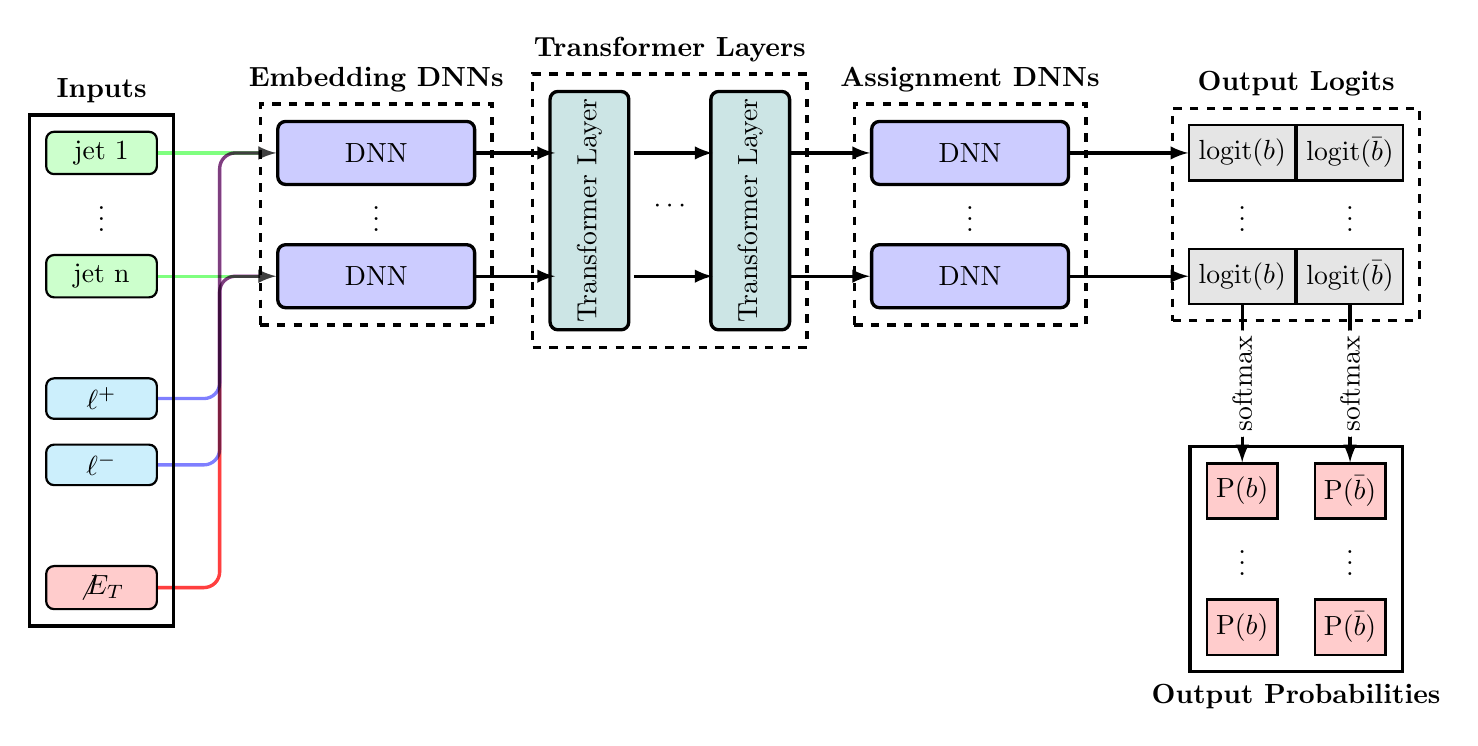
\begin{tikzpicture}[
    >=LaTeX, % Use default LaTeX arrows
    very thick,
    arrow/.style={
        -latex,
        very thick,
        rounded corners=0.2cm
    },
    block/.style={
        rectangle,
        fill=gray!10,
        rounded corners=3mm,
        draw,
        very thick
    },
    dnn_block/.style={
        rectangle,
        fill=blue!20,
        rounded corners=1mm,
        inner xsep=0em,
        inner ysep=0.25em,
        minimum height=1.4em,
        align=center,
        text width=2.5cm,
        draw,
        very thick
    },
    transformer_layer/.style={
        rectangle,
        fill=teal!20,
        rounded corners=1mm,
        inner xsep=0em,
        inner ysep=0.25em,
        minimum height=1cm,
        align=center,
        %text width=2.5cm,
        draw,
        very thick
    },
    input/.style={ % Input or output node
        rectangle,
        minimum width=4em,
        rounded corners=1mm,
        draw,
        fill=green!20,
        thick
    },
    output/.style={ % Input or output node
        rectangle,
        minimum width=2.25em,
        draw,
        fill=red!20,
        thick
    }
]

% Input nodes
\node[input] (jet_1) {jet 1};
\node[input, below=1cm of jet_1] (jet_n) {jet n};
\node[yshift=0.05cm] at ($(jet_1)!0.5!(jet_n)$, yshift=-0.1cm) (jet_dots1) {$\vdots$};


\node[input,fill=cyan!20, below=1cm of jet_n] (lepton_1) {$\ell^+$};
\node[input,fill=cyan!20, below=0.3cm of lepton_1] (lepton_2) {$\ell^-$};

\node[input,fill=red!20, below=1cm of lepton_2] (met) {$\not{E}_T$};

% Input Embeddings
\node[dnn_block, right=1.5cm of jet_1, minimum height = 0.8cm] (dnn_1) {DNN};
\node[dnn_block, right=1.5cm of jet_n, minimum height = 0.8cm] (dnn_n) {DNN};
\node[yshift=0.05cm] at ($(dnn_1)!0.5!(dnn_n)$) (dnn_dots) {$\vdots$};

% Transformer Layers (perpendicular, rotated text)
\node[transformer_layer, 
      right=2cm of dnn_dots, 
      minimum height=3cm, 
      minimum width=1cm] 
      (transformer_1) {\rotatebox{90}{Transformer Layer}};

\node[transformer_layer, 
      right=1cm of transformer_1, 
      minimum height=3cm, 
      minimum width=1cm] 
      (transformer_n) {\rotatebox{90}{Transformer Layer}};
\node[yshift=0.05cm] at ($(transformer_1)!0.5!(transformer_n)$) (transformer_dots) {$\cdots$};

% Assignment DNNs
\node[dnn_block, right=5cm of dnn_1, minimum height = 0.8cm] (assign_1) {DNN};
\node[dnn_block, right=5cm of dnn_n, minimum height = 0.8cm] (assign_n) {DNN};
\node[yshift=0.05cm] at ($(assign_1)!0.5!(assign_n)$) (assign_dots) {$\vdots$};

% Output Logits
\node[output, fill=gray!20, right=1.5cm of assign_1, minimum height = 0.7cm] (output_b_1) {logit($b$)};
\node[output, fill=gray!20, right=1.5cm of assign_n, minimum height = 0.7cm] (output_b_n) {logit($b$)};
\node[yshift=0.05cm] at ($(output_b_1)!0.5!(output_b_n)$) (output_dots) {$\vdots$};
\node[output, fill=gray!20, right=0cm of output_b_1, minimum height = 0.7cm] (output_bbar_1) {logit($\bar{b}$)};
\node[output, fill=gray!20, right=0cm of output_b_n, minimum height = 0.7cm] (output_bbar_n) {logit($\bar{b}$)};
\node[yshift=0.05cm] at ($(output_bbar_1)!0.5!(output_bbar_n)$) (output_dots) {$\vdots$};

% Output Probabilities
\node[output, below=2cm of output_b_n, minimum height = 0.7cm] (prob_b_1) {P($b$)};
\node[output, below=2cm of output_bbar_n, minimum height = 0.7cm] (prob_bbar_1) {P($\bar{b}$)};
\node[output, below=1cm of prob_b_1, minimum height = 0.7cm] (prob_b_n) {P($b$)};
\node[output, below=1cm of prob_bbar_1, minimum height = 0.7cm] (prob_bbar_n) {P($\bar{b}$)};
\node[yshift=0.05cm] at ($(prob_b_1)!0.5!(prob_b_n)$) (prob_dots) {$\vdots$};
\node[yshift=0.05cm] at ($(prob_bbar_1)!0.5!(prob_bbar_n)$) (prob_dots) {$\vdots$};


% 
\node[fit=(jet_1)(jet_n)(lepton_1)(lepton_2)(met), 
      draw, 
      inner sep=0.2cm, 
      label=above:{\textbf{Inputs}}] 
      (input_box) {};

\node[fit=(dnn_1)(dnn_n), 
      draw, 
      dashed, 
      inner sep=0.2cm, 
      label=above:{\textbf{Embedding DNNs}}] 
      (embedding_box) {};

\node[fit=(transformer_1)(transformer_n), 
      draw, 
      dashed, 
      inner sep=0.2cm, 
      label=above:{\textbf{Transformer Layers}}] 
      (transformer_box) {};

\node[fit=(assign_1)(assign_n), 
      draw, 
      dashed, 
      inner sep=0.2cm, 
      label=above:{\textbf{Assignment DNNs}}] 
      (assignment_box) {};
    
\node[fit=(output_b_1)(output_b_n)(output_bbar_1)(output_bbar_n), 
      draw, 
      dashed, 
      inner sep=0.2cm, 
      label=above:{\textbf{Output Logits}}] 
      (logit_box) {};

\node[fit=(prob_b_1)(prob_b_n)(prob_bbar_1)(prob_bbar_n), 
      draw, 
      very thick, 
      inner sep=0.2cm, 
      label=below:{\textbf{Output Probabilities}}] 
      (probability_box) {};
    


% Arrows from inputs to embeddings
\draw[arrow, color=green, opacity=0.5, blend mode=multiply] (jet_1) -- (dnn_1);
\draw[arrow, color=green, opacity=0.5, blend mode=multiply] (jet_n) -- (dnn_n);
\draw[arrow, color=blue, opacity=0.5, blend mode=multiply] (lepton_1) -- ++(1.5,0) |- (dnn_1.west);
\draw[arrow, color=blue, opacity=0.5, blend mode=multiply] (lepton_2) -- ++(1.5,0) |- (dnn_n.west);
\draw[arrow, color=red, opacity=0.5, blend mode=multiply] (met) -- ++(1.5,0) |- (dnn_1.west);
\draw[arrow, color=red, opacity=0.5, blend mode=multiply] (met) -- ++(1.5,0) |- (dnn_n.west);

% Arrows from embeddings to transformer
\draw[arrow] (dnn_1.east) -- ++(1,0);
\draw[arrow] (dnn_n.east) -- ++(1,0);

% Arrows through transformer layers
\draw [arrow] ($(dnn_1.east) + (2,0)$) -- ($(dnn_1.east) + (3,0)$);
\draw [arrow] ($(dnn_n.east) + (2,0)$) -- ($(dnn_n.east) + (3,0)$);

% Arrows from transformer to assignment DNNs
\draw[arrow] ($(dnn_1.east) + (4,0)$) -- (assign_1.west);
\draw[arrow] ($(dnn_n.east) + (4,0)$) -- (assign_n.west);

% Arrows from assignment DNNs to outputs
\draw[arrow] (assign_1.east) -- (output_b_1.west);
\draw[arrow] (assign_n.east) -- (output_b_n.west);

% Arrows from logits to probabilities
\draw[arrow] (output_b_n.south) -- (prob_b_1.north) node[midway, fill=white, inner sep=2pt] {\rotatebox{90}{softmax}};
\draw[arrow] (output_bbar_n.south) -- (prob_bbar_1.north) node[midway, fill=white, inner sep=2pt] {\rotatebox{90}{softmax}};
\end{tikzpicture}
\end{document}